\chapter{Detecting corruption, collusion \& fraud:\\ Data product}\label{chap_prod}

\section{Data pipeline}
\begin{figure}[H]
\begin{center}
\caption{Data pipeline}
\label{fig_pipeline}
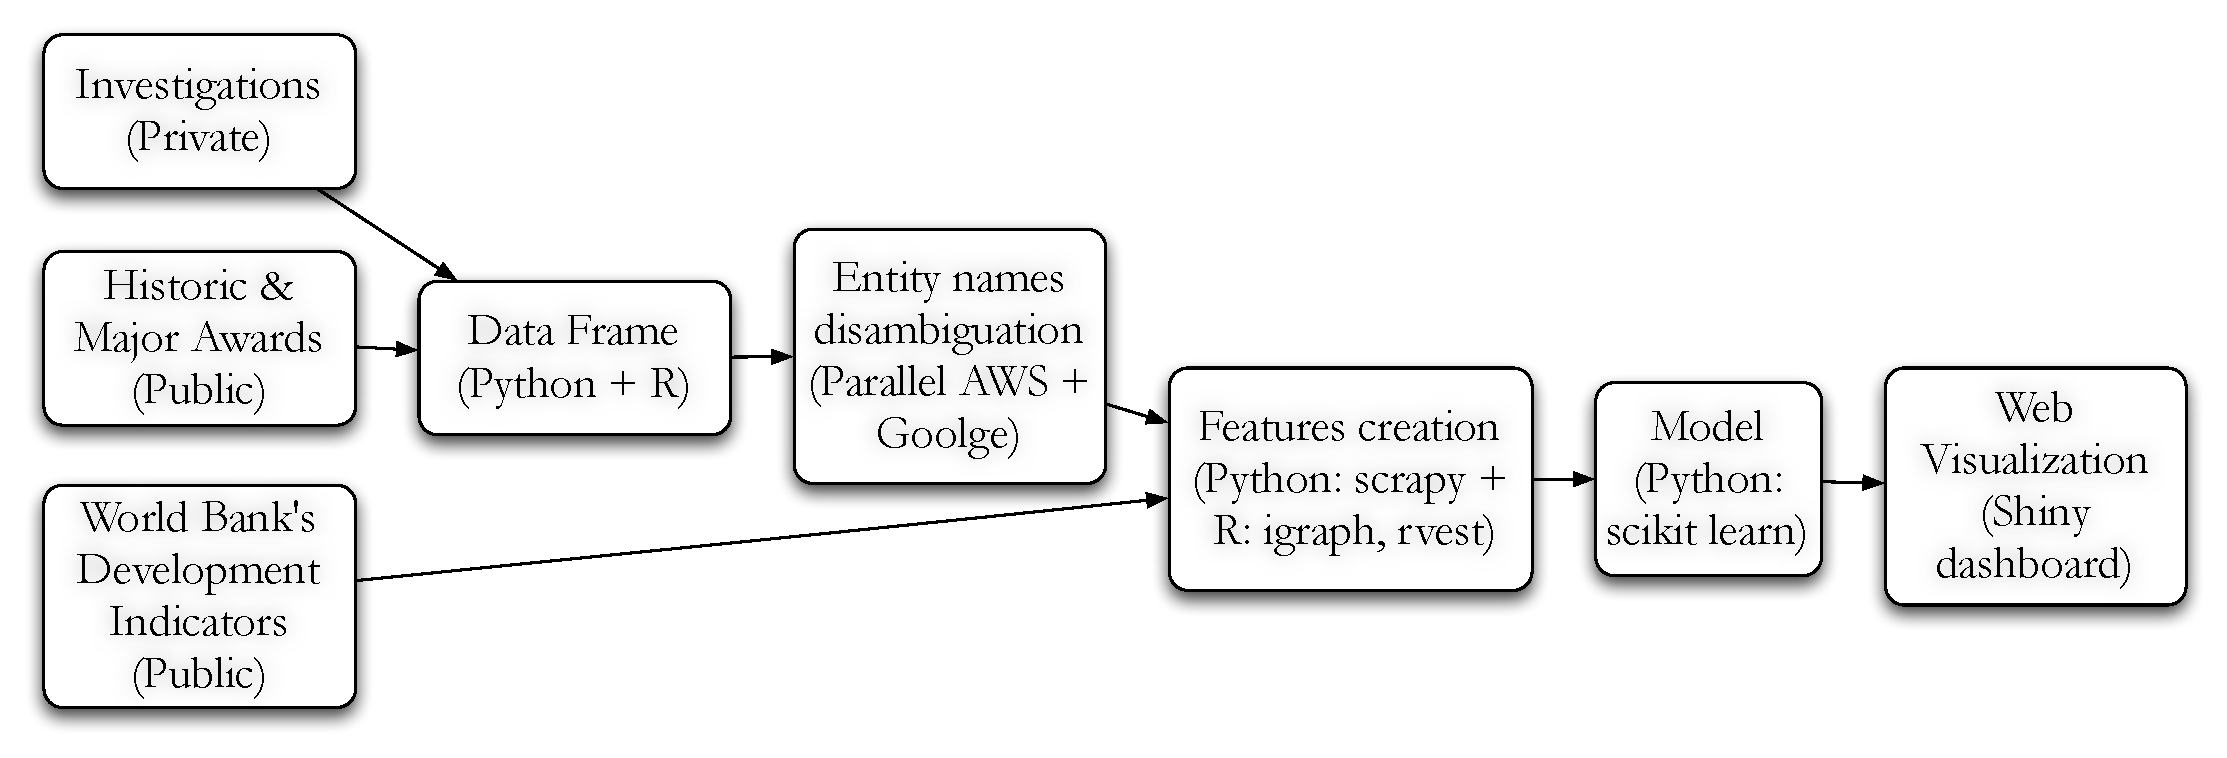
\includegraphics[width=\textwidth,height=1\textheight,keepaspectratio]{../img/pipeline.pdf}
\end{center}
\noindent \footnotesize{\textbf{Source:} Own creation.}
\end{figure}

\section{Model}

\section{Web visualization application: dashboard}

\subsection{Dashboard outline}

\subsection{Interactive map}

\begin{figure}[H]
\begin{center}
\caption{Interactive map}
\label{fig_interactive_map}
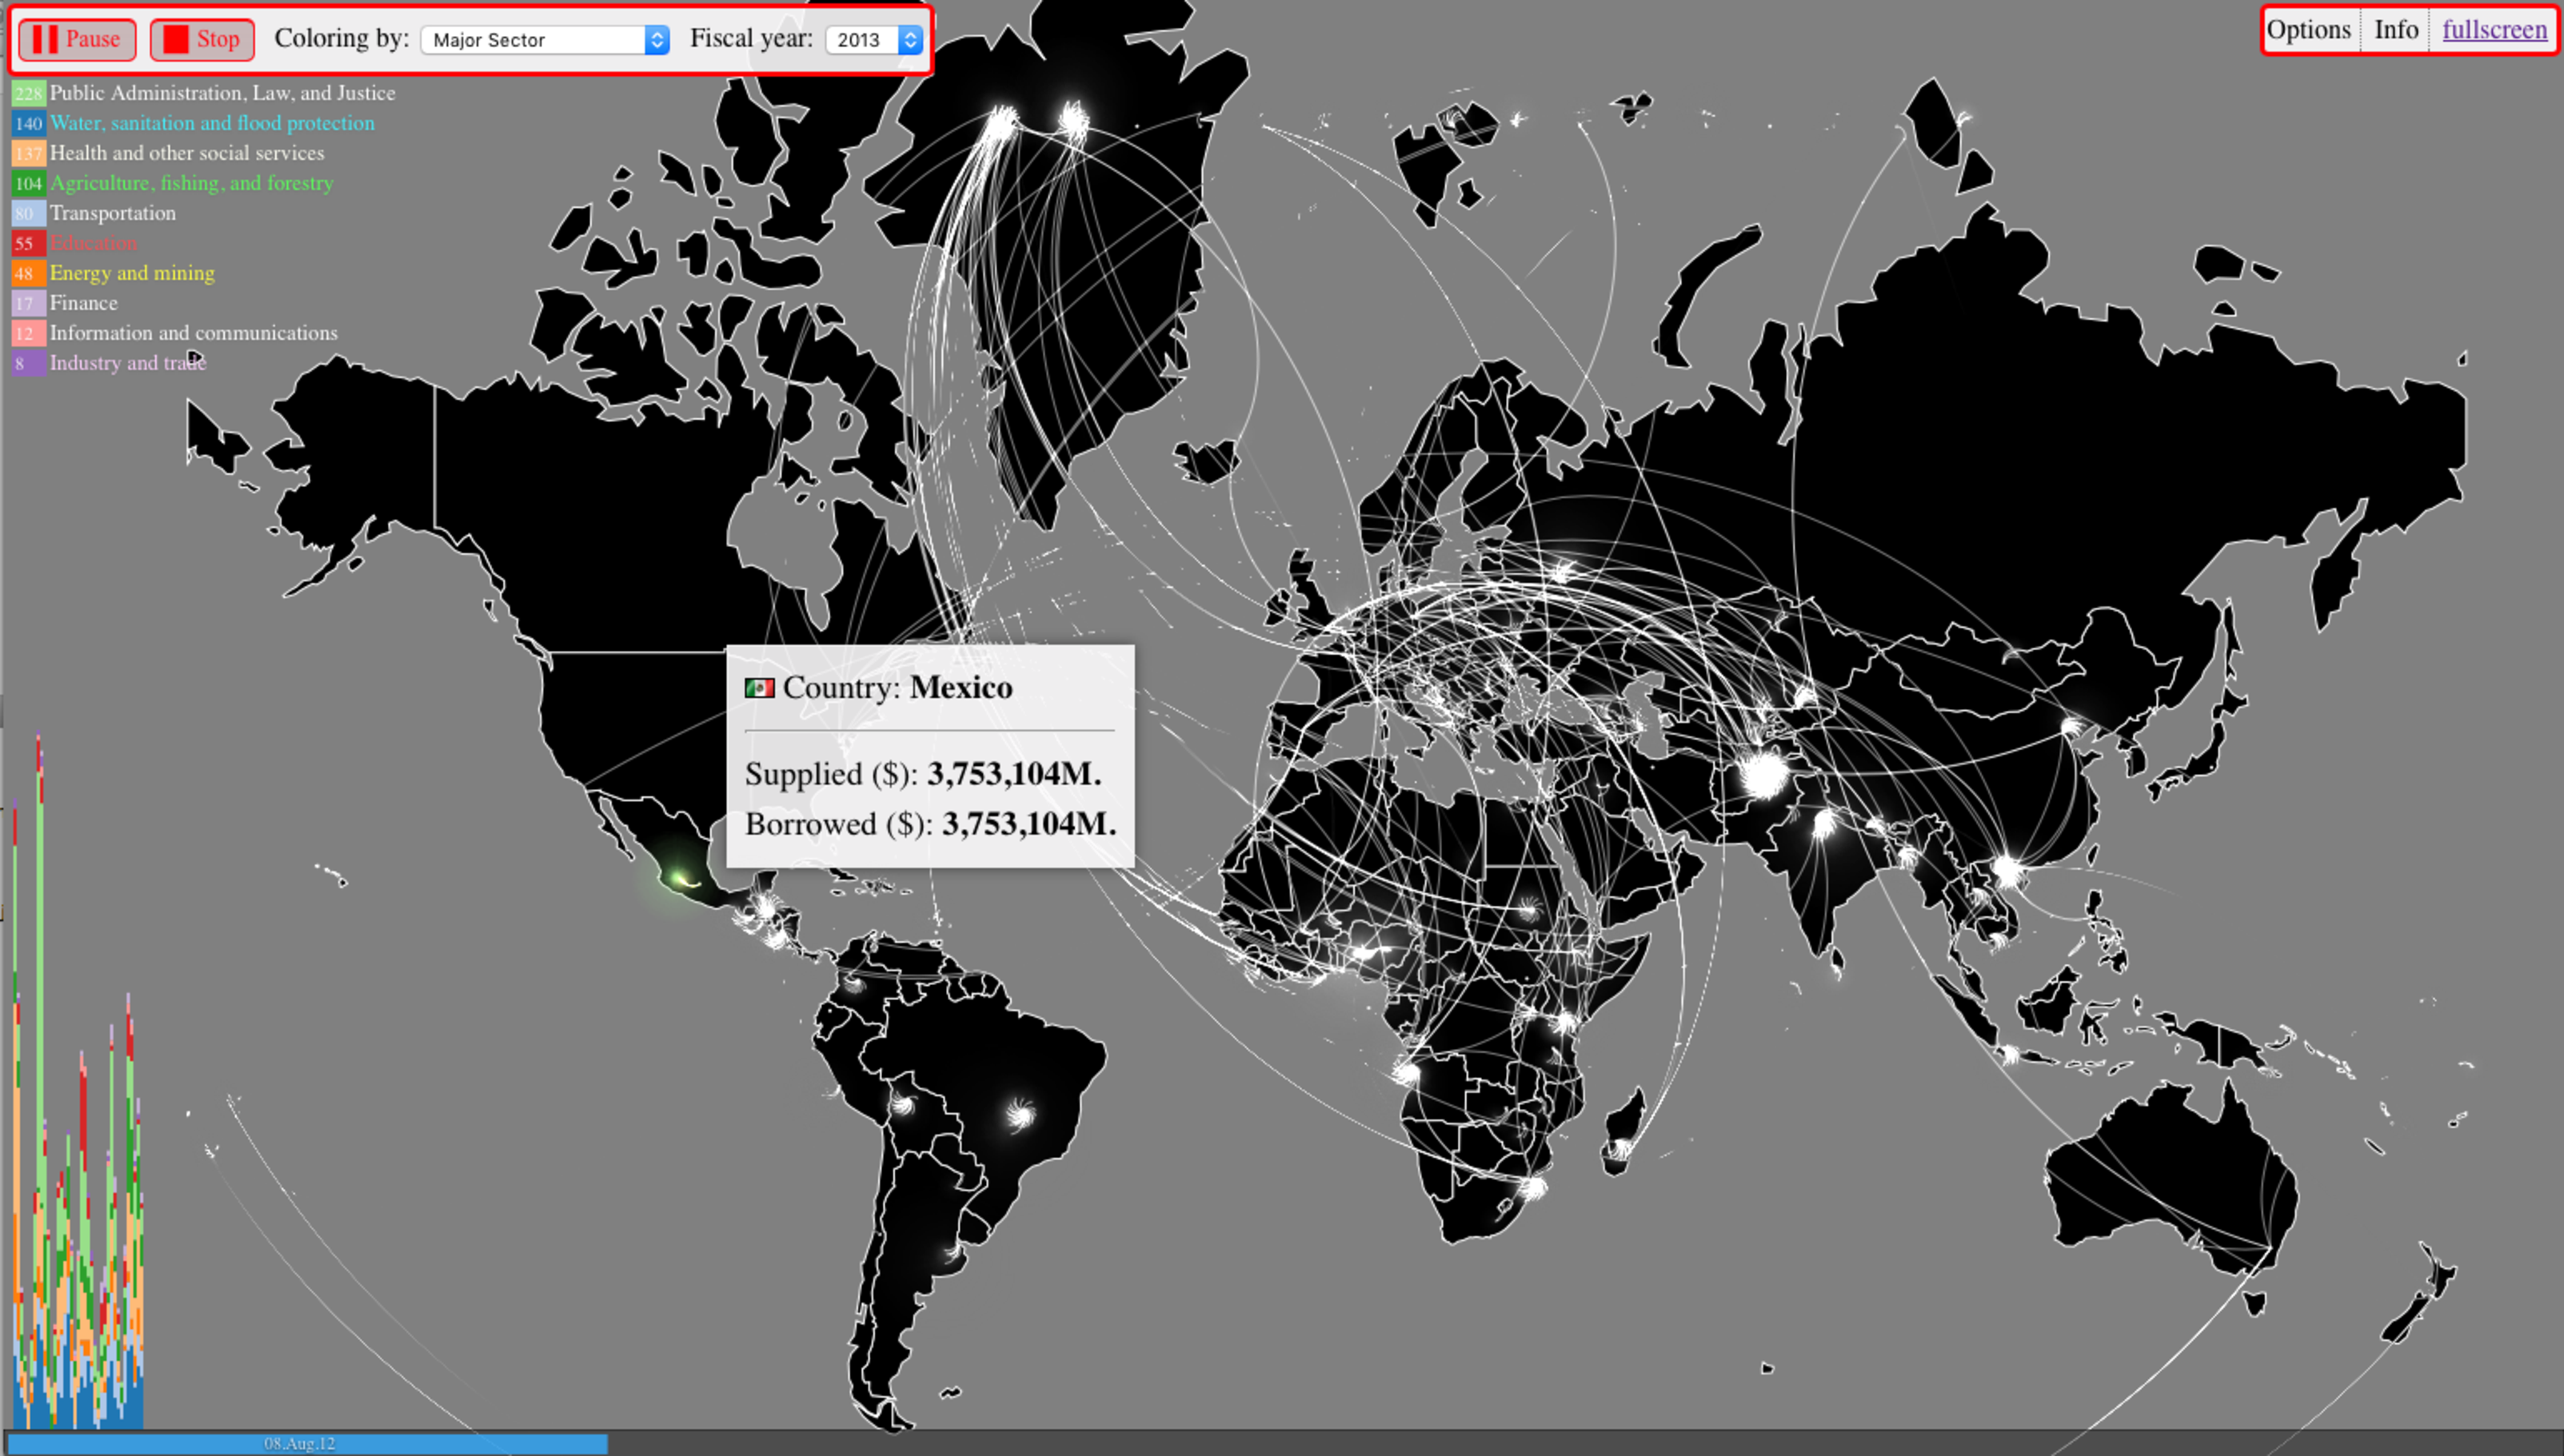
\includegraphics[width=\textwidth,height=1\textheight,keepaspectratio]{../img/interactive_map_mex.pdf}
\end{center}
\noindent \footnotesize{\textbf{Source:} Own creation based on \cite{wb_i_map}. \\Go to \href{http://detecting-corruption.carlospetricioli.com/interactive_map}{detecting-corruption.carlospetricioli.com/interactive\_map} to see a live version. \\Data from the World Bank \parencite{wb_data}.}
\end{figure}

\subsection{Companies \& projects network}

\subsection{Contract specific risk map}

\begin{figure}[H]
\begin{center}
\caption{Risk map (Sample)}
\label{fig_risk_map}
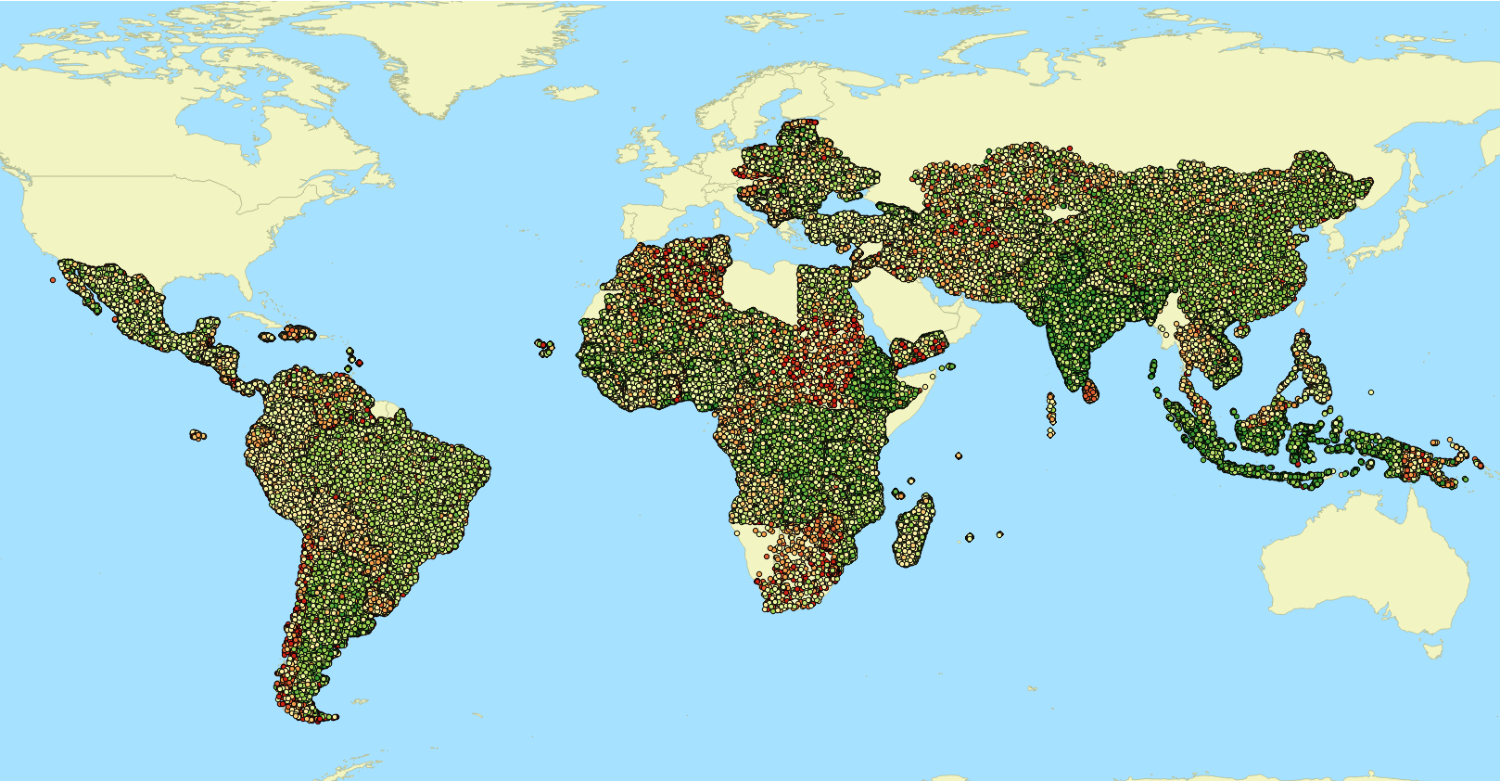
\includegraphics[width=\textwidth,height=1\textheight,keepaspectratio]{../img/risk_map.pdf}
\end{center}
\noindent \footnotesize{\textbf{Source:} Own creation based on \cite{wb_i_map}. \\Data from the World Bank \parencite{wb_data}.}
\end{figure}

